\documentclass{ximera}

%\usepackage{todonotes}

\newcommand{\todo}{}

\usepackage{esint} % for \oiint
\ifxake%%https://math.meta.stackexchange.com/questions/9973/how-do-you-render-a-closed-surface-double-integral
\renewcommand{\oiint}{{\large\bigcirc}\kern-1.56em\iint}
\fi


\graphicspath{
  {./}
  {ximeraTutorial/}
  {basicPhilosophy/}
  {functionsOfSeveralVariables/}
  {normalVectors/}
  {lagrangeMultipliers/}
  {vectorFields/}
  {greensTheorem/}
  {shapeOfThingsToCome/}
  {dotProducts/}
  {partialDerivativesAndTheGradientVector/}
  {../productAndQuotientRules/exercises/}
  {../normalVectors/exercisesParametricPlots/}
  {../continuityOfFunctionsOfSeveralVariables/exercises/}
  {../partialDerivativesAndTheGradientVector/exercises/}
  {../directionalDerivativeAndChainRule/exercises/}
  {../commonCoordinates/exercisesCylindricalCoordinates/}
  {../commonCoordinates/exercisesSphericalCoordinates/}
  {../greensTheorem/exercisesCurlAndLineIntegrals/}
  {../greensTheorem/exercisesDivergenceAndLineIntegrals/}
  {../shapeOfThingsToCome/exercisesDivergenceTheorem/}
  {../greensTheorem/}
  {../shapeOfThingsToCome/}
  {../separableDifferentialEquations/exercises/}
  {vectorFields/}
}

\newcommand{\mooculus}{\textsf{\textbf{MOOC}\textnormal{\textsf{ULUS}}}}

\usepackage{tkz-euclide}
\usepackage{tikz}
\usepackage{tikz-cd}
\usetikzlibrary{arrows}
\tikzset{>=stealth,commutative diagrams/.cd,
  arrow style=tikz,diagrams={>=stealth}} %% cool arrow head
\tikzset{shorten <>/.style={ shorten >=#1, shorten <=#1 } } %% allows shorter vectors

\usetikzlibrary{backgrounds} %% for boxes around graphs
\usetikzlibrary{shapes,positioning}  %% Clouds and stars
\usetikzlibrary{matrix} %% for matrix
\usepgfplotslibrary{polar} %% for polar plots
\usepgfplotslibrary{fillbetween} %% to shade area between curves in TikZ
%\usetkzobj{all}
\usepackage[makeroom]{cancel} %% for strike outs
%\usepackage{mathtools} %% for pretty underbrace % Breaks Ximera
%\usepackage{multicol}
\usepackage{pgffor} %% required for integral for loops



%% http://tex.stackexchange.com/questions/66490/drawing-a-tikz-arc-specifying-the-center
%% Draws beach ball
\tikzset{pics/carc/.style args={#1:#2:#3}{code={\draw[pic actions] (#1:#3) arc(#1:#2:#3);}}}



\usepackage{array}
\setlength{\extrarowheight}{+.1cm}
\newdimen\digitwidth
\settowidth\digitwidth{9}
\def\divrule#1#2{
\noalign{\moveright#1\digitwidth
\vbox{\hrule width#2\digitwidth}}}




% \newcommand{\RR}{\mathbb R}
% \newcommand{\R}{\mathbb R}
% \newcommand{\N}{\mathbb N}
% \newcommand{\Z}{\mathbb Z}

\newcommand{\sagemath}{\textsf{SageMath}}


%\renewcommand{\d}{\,d\!}
%\renewcommand{\d}{\mathop{}\!d}
%\newcommand{\dd}[2][]{\frac{\d #1}{\d #2}}
%\newcommand{\pp}[2][]{\frac{\partial #1}{\partial #2}}
% \renewcommand{\l}{\ell}
%\newcommand{\ddx}{\frac{d}{\d x}}

% \newcommand{\zeroOverZero}{\ensuremath{\boldsymbol{\tfrac{0}{0}}}}
%\newcommand{\inftyOverInfty}{\ensuremath{\boldsymbol{\tfrac{\infty}{\infty}}}}
%\newcommand{\zeroOverInfty}{\ensuremath{\boldsymbol{\tfrac{0}{\infty}}}}
%\newcommand{\zeroTimesInfty}{\ensuremath{\small\boldsymbol{0\cdot \infty}}}
%\newcommand{\inftyMinusInfty}{\ensuremath{\small\boldsymbol{\infty - \infty}}}
%\newcommand{\oneToInfty}{\ensuremath{\boldsymbol{1^\infty}}}
%\newcommand{\zeroToZero}{\ensuremath{\boldsymbol{0^0}}}
%\newcommand{\inftyToZero}{\ensuremath{\boldsymbol{\infty^0}}}



% \newcommand{\numOverZero}{\ensuremath{\boldsymbol{\tfrac{\#}{0}}}}
% \newcommand{\dfn}{\textbf}
% \newcommand{\unit}{\,\mathrm}
% \newcommand{\unit}{\mathop{}\!\mathrm}
% \newcommand{\eval}[1]{\bigg[ #1 \bigg]}
% \newcommand{\seq}[1]{\left( #1 \right)}
% \renewcommand{\epsilon}{\varepsilon}
% \renewcommand{\phi}{\varphi}


% \renewcommand{\iff}{\Leftrightarrow}

% \DeclareMathOperator{\arccot}{arccot}
% \DeclareMathOperator{\arcsec}{arcsec}
% \DeclareMathOperator{\arccsc}{arccsc}
% \DeclareMathOperator{\si}{Si}
% \DeclareMathOperator{\scal}{scal}
% \DeclareMathOperator{\sign}{sign}


%% \newcommand{\tightoverset}[2]{% for arrow vec
%%   \mathop{#2}\limits^{\vbox to -.5ex{\kern-0.75ex\hbox{$#1$}\vss}}}
% \newcommand{\arrowvec}[1]{{\overset{\rightharpoonup}{#1}}}
% \renewcommand{\vec}[1]{\arrowvec{\mathbf{#1}}}
% \renewcommand{\vec}[1]{{\overset{\boldsymbol{\rightharpoonup}}{\mathbf{#1}}}}

% \newcommand{\point}[1]{\left(#1\right)} %this allows \vector{ to be changed to \vector{ with a quick find and replace
% \newcommand{\pt}[1]{\mathbf{#1}} %this allows \vec{ to be changed to \vec{ with a quick find and replace
% \newcommand{\Lim}[2]{\lim_{\point{#1} \to \point{#2}}} %Bart, I changed this to point since I want to use it.  It runs through both of the exercise and exerciseE files in limits section, which is why it was in each document to start with.

% \DeclareMathOperator{\proj}{\mathbf{proj}}
% \newcommand{\veci}{{\boldsymbol{\hat{\imath}}}}
% \newcommand{\vecj}{{\boldsymbol{\hat{\jmath}}}}
% \newcommand{\veck}{{\boldsymbol{\hat{k}}}}
% \newcommand{\vecl}{\vec{\boldsymbol{\l}}}
% \newcommand{\uvec}[1]{\mathbf{\hat{#1}}}
% \newcommand{\utan}{\mathbf{\hat{t}}}
% \newcommand{\unormal}{\mathbf{\hat{n}}}
% \newcommand{\ubinormal}{\mathbf{\hat{b}}}

% \newcommand{\dotp}{\bullet}
% \newcommand{\cross}{\boldsymbol\times}
% \newcommand{\grad}{\boldsymbol\nabla}
% \newcommand{\divergence}{\grad\dotp}
% \newcommand{\curl}{\grad\cross}
%\DeclareMathOperator{\divergence}{divergence}
%\DeclareMathOperator{\curl}[1]{\grad\cross #1}
% \newcommand{\lto}{\mathop{\longrightarrow\,}\limits}

% \renewcommand{\bar}{\overline}

\colorlet{textColor}{black}
\colorlet{background}{white}
\colorlet{penColor}{blue!50!black} % Color of a curve in a plot
\colorlet{penColor2}{red!50!black}% Color of a curve in a plot
\colorlet{penColor3}{red!50!blue} % Color of a curve in a plot
\colorlet{penColor4}{green!50!black} % Color of a curve in a plot
\colorlet{penColor5}{orange!80!black} % Color of a curve in a plot
\colorlet{penColor6}{yellow!70!black} % Color of a curve in a plot
\colorlet{fill1}{penColor!20} % Color of fill in a plot
\colorlet{fill2}{penColor2!20} % Color of fill in a plot
\colorlet{fillp}{fill1} % Color of positive area
\colorlet{filln}{penColor2!20} % Color of negative area
\colorlet{fill3}{penColor3!20} % Fill
\colorlet{fill4}{penColor4!20} % Fill
\colorlet{fill5}{penColor5!20} % Fill
\colorlet{gridColor}{gray!50} % Color of grid in a plot

\newcommand{\surfaceColor}{violet}
\newcommand{\surfaceColorTwo}{redyellow}
\newcommand{\sliceColor}{greenyellow}




\pgfmathdeclarefunction{gauss}{2}{% gives gaussian
  \pgfmathparse{1/(#2*sqrt(2*pi))*exp(-((x-#1)^2)/(2*#2^2))}%
}


%%%%%%%%%%%%%
%% Vectors
%%%%%%%%%%%%%

%% Simple horiz vectors
\renewcommand{\vector}[1]{\left\langle #1\right\rangle}


%% %% Complex Horiz Vectors with angle brackets
%% \makeatletter
%% \renewcommand{\vector}[2][ , ]{\left\langle%
%%   \def\nextitem{\def\nextitem{#1}}%
%%   \@for \el:=#2\do{\nextitem\el}\right\rangle%
%% }
%% \makeatother

%% %% Vertical Vectors
%% \def\vector#1{\begin{bmatrix}\vecListA#1,,\end{bmatrix}}
%% \def\vecListA#1,{\if,#1,\else #1\cr \expandafter \vecListA \fi}

%%%%%%%%%%%%%
%% End of vectors
%%%%%%%%%%%%%

%\newcommand{\fullwidth}{}
%\newcommand{\normalwidth}{}



%% makes a snazzy t-chart for evaluating functions
%\newenvironment{tchart}{\rowcolors{2}{}{background!90!textColor}\array}{\endarray}

%%This is to help with formatting on future title pages.
\newenvironment{sectionOutcomes}{}{}



%% Flowchart stuff
%\tikzstyle{startstop} = [rectangle, rounded corners, minimum width=3cm, minimum height=1cm,text centered, draw=black]
%\tikzstyle{question} = [rectangle, minimum width=3cm, minimum height=1cm, text centered, draw=black]
%\tikzstyle{decision} = [trapezium, trapezium left angle=70, trapezium right angle=110, minimum width=3cm, minimum height=1cm, text centered, draw=black]
%\tikzstyle{question} = [rectangle, rounded corners, minimum width=3cm, minimum height=1cm,text centered, draw=black]
%\tikzstyle{process} = [rectangle, minimum width=3cm, minimum height=1cm, text centered, draw=black]
%\tikzstyle{decision} = [trapezium, trapezium left angle=70, trapezium right angle=110, minimum width=3cm, minimum height=1cm, text centered, draw=black]


\title{iRoC}

\begin{document}

\begin{abstract}
rate of change
\end{abstract}
\maketitle




By function \textbf{behavior}, we mean the rate of change.


We have two flavors of this.




\begin{fact} \textbf{\textcolor{blue!55!black}{Over an Interval}}    \\


The rate of change of the function $f$ over the interval $[a, b]$ is given by $\frac{f(b) - f(a)}{b - a}$. \\


This is our algebraic version of rate of change. This is also referred to as the \textit{average rate of change} over the interval $[a, b]$.


\end{fact}






\begin{fact} \textbf{\textcolor{blue!55!black}{At a Domain Number}}   \\


The rate of change of the function $f$ at the domain number $a$ is given by the slope of the tangent line at the point $(a, f(a))$ on the graph. \\


This rate of change is known as the \textbf{\textcolor{purple!85!blue}{instantaneous rate of change of f at a}} and is measured by the \textbf{\textcolor{blue!55!black}{derivative of f at a}}. 


This is our Calculus version of rate of change.


\end{fact}


Each is a different measurement of the change in a function's value compared to changes in the domain. \\




\begin{notation} the \textbf{\textcolor{blue!55!black}{derivative of f at a}}

\begin{center}
\textbf{\textcolor{blue!55!black}{$iRoC_f(a)$}} or \textbf{\textcolor{blue!55!black}{$f'(a)$}} 
\end{center}

\end{notation}









Algebra describes the change from one domain number to another. It describes function change over an interval. Calculus takes an extreme viewpoint on this.  Calculus asks about the interval $[a,a]$. Algebra doesn't know what to do with this type of interval. The rate of change of a function at one domain number, $a$, makes no sense, algebraically. Calculus makes sense of it as the slope of a tangent line at $(a, f(a))$. \\

This gives us two types of interpretations for increasing and decreasing. \\


\textbf{\textcolor{red!80!black}{$\blacktriangleright$ Algebraic Increasing}} \\



The function, $f$, is \textbf{\textcolor{purple!85!blue}{increasing on the interval}} $[a, b]$ if


\[
f(c) \leq f(d) \, \text{ whenever } \, c \leq d \, \text{ for all } \, c, d \in [a,b]
\]









\textbf{\textcolor{red!80!black}{$\blacktriangleright$ Calculus Increasing}} \\



The function, $f$, is \textbf{\textcolor{purple!85!blue}{increasing at a}} if


\[
iRoC_f(a) > 0 \, \text{ or } \, f'(a) > 0
\]










\textbf{\textcolor{red!80!black}{$\blacktriangleright$ Algebraic Decreasing}} \\



The function, $f$, is \textbf{\textcolor{purple!85!blue}{decreasing on the interval}} $[a, b]$ if


\[
f(c) \geq f(d) \, \text{ whenever } \, c \leq d \, \text{ for all } \, c, d \in [a,b]
\]









\textbf{\textcolor{red!80!black}{$\blacktriangleright$ Calculus Decreasing}} \\



The function, $f$, is \textbf{\textcolor{purple!85!blue}{decreasing at a}} if


\[
iRoC_f(a) < 0 \, \text{ or } \, f'(a) < 0
\]








The instantaneous rate of change can have a value at each domain number, which makes it into a function.






\section*{iRoC}


The instantaneous rate of change (a.k.a the derivative) gives us a formula for the slopes of tangent lines, which are rates of change.



\textbf{\textcolor{red!90!darkgray}{$\blacktriangleright$}} From vertex form, $f(x) = a (x -h)^2 + k$, we have $iRoC_f(x) = f'(x) = 2 a \, (x-h)$. \\



\textbf{\textcolor{red!90!darkgray}{$\blacktriangleright$}} From standard form, $f(x) = a \, x^2 + b \, x + c$, we have $iRoC_f(x) = f'(x) = 2 a \, x + b$. \\



















\begin{example}


Let $M(t) = -\frac{1}{2} (t - 3)^2 + 5$ \\

What is the maximum value of $M(t)$? \\



\begin{explanation}

From the vertex form, we can see a negative leading coefficient, which tells us the parabola will open down, that $M$ increases and then decreases, and that there is a maximum value. \\

From the vertex form, we can tell that the highest point on the graph is $(3, 5)$, which tells us that the maximum value of $M$ is $5$ and it occurs at $3$.



\begin{image}
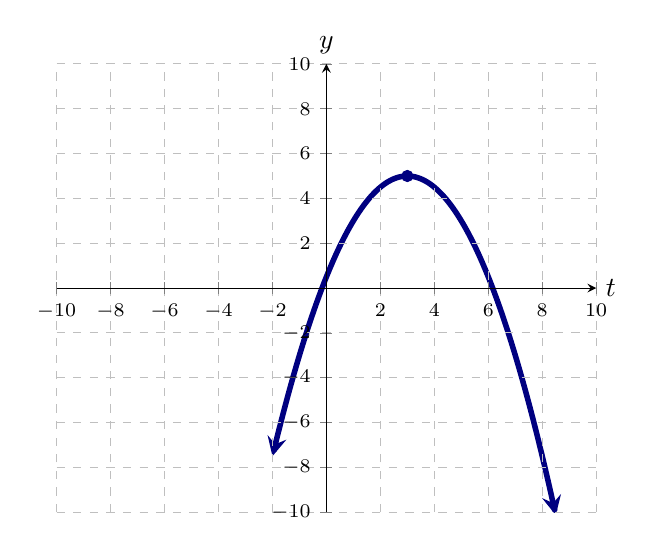
\begin{tikzpicture}
  \begin{axis}[
            domain=-10:10, ymax=10, xmax=10, ymin=-10, xmin=-10,
            axis lines =center, xlabel=$t$, ylabel={$y$}, grid = major, grid style={dashed},
            ytick={-10,-8,-6,-4,-2,2,4,6,8,10},
            xtick={-10,-8,-6,-4,-2,2,4,6,8,10},
            yticklabels={$-10$,$-8$,$-6$,$-4$,$-2$,$2$,$4$,$6$,$8$,$10$}, 
            xticklabels={$-10$,$-8$,$-6$,$-4$,$-2$,$2$,$4$,$6$,$8$,$10$},
            ticklabel style={font=\scriptsize},
            every axis y label/.style={at=(current axis.above origin),anchor=south},
            every axis x label/.style={at=(current axis.right of origin),anchor=west},
            axis on top
          ]
          
          %\addplot [line width=2, penColor2, smooth,samples=100,domain=(-6:2)] {-2*x-3};
          \addplot [line width=2, penColor, smooth,samples=200,domain=(-2:8.5),<->] {-0.5*(x-3)^2 + 5};
          %\addplot [line width=2, penColor2, smooth,samples=200,domain=(-4:4),<->] {2*(x-1)+3};

          %\addplot[color=penColor,fill=penColor2,only marks,mark=*] coordinates{(-6,9)};
          %\addplot[color=penColor,fill=penColor2,only marks,mark=*] coordinates{(2,-7)};

          \addplot[color=penColor,fill=penColor,only marks,mark=*] coordinates{(3,5)};
          %\addplot[color=penColor,fill=penColor,only marks,mark=*] coordinates{(-0.162,0)};
          %\addplot[color=penColor,fill=penColor,only marks,mark=*] coordinates{(6.162,0)};



           

  \end{axis}
\end{tikzpicture}
\end{image}


\end{explanation}
\end{example}



















\begin{example}


Let $M(t) = -\frac{1}{2} (t - 3)^2 + 5$ \\

What is the maximum value of $M(t)$? \\



\begin{explanation}

From the vertex form, we have $iRoC_M(t) = -(t - 3)$ or $M'(t) = -(t - 3) = -t + 3 = 3 - t$. \\



The $iRoC$ or derivative is itself a function.  We could plot its graph. For a quadratic function, the derivative is a linear function whose graph is a line.




Graph of $y = iRoC_M(t) = M'(t) = 3 - t$







\begin{image}
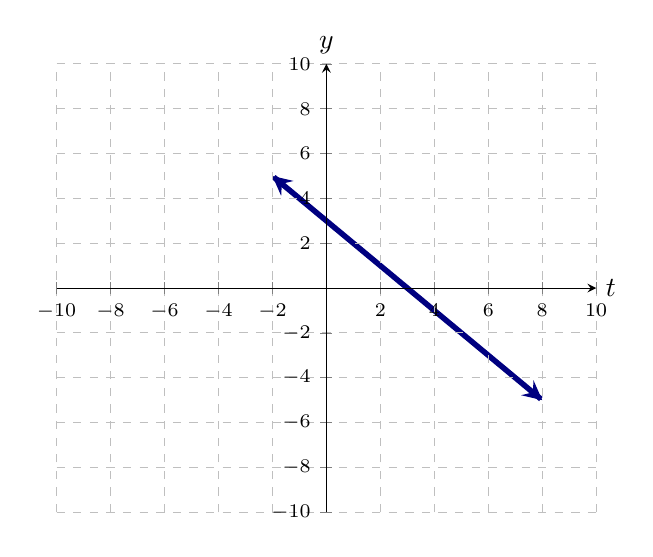
\begin{tikzpicture}
  \begin{axis}[
            domain=-10:10, ymax=10, xmax=10, ymin=-10, xmin=-10,
            axis lines =center, xlabel=$t$, ylabel={$y$}, grid = major, grid style={dashed},
            ytick={-10,-8,-6,-4,-2,2,4,6,8,10},
            xtick={-10,-8,-6,-4,-2,2,4,6,8,10},
            yticklabels={$-10$,$-8$,$-6$,$-4$,$-2$,$2$,$4$,$6$,$8$,$10$}, 
            xticklabels={$-10$,$-8$,$-6$,$-4$,$-2$,$2$,$4$,$6$,$8$,$10$},
            ticklabel style={font=\scriptsize},
            every axis y label/.style={at=(current axis.above origin),anchor=south},
            every axis x label/.style={at=(current axis.right of origin),anchor=west},
            axis on top
          ]
          
          %\addplot [line width=2, penColor2, smooth,samples=100,domain=(-6:2)] {-2*x-3};
          \addplot [line width=2, penColor, smooth,samples=200,domain=(-2:8),<->] {-x+3};
          %\addplot [line width=2, penColor2, smooth,samples=200,domain=(-4:4),<->] {2*(x-1)+3};

          %\addplot[color=penColor,fill=penColor2,only marks,mark=*] coordinates{(-6,9)};
          %\addplot[color=penColor,fill=penColor2,only marks,mark=*] coordinates{(2,-7)};

          %\addplot[color=penColor,fill=penColor,only marks,mark=*] coordinates{(1,3)};
          %\addplot[color=penColor,fill=penColor,only marks,mark=*] coordinates{(-0.162,0)};
          %\addplot[color=penColor,fill=penColor,only marks,mark=*] coordinates{(6.162,0)};



           

  \end{axis}
\end{tikzpicture}
\end{image}


The derivative is positive on $(-\infty, 3)$, which tells us that the tangent lines to the parabola have positive slopes for the left half of the parabola. This tells us that $M$ is \wordChoice{\choice[correct]{increasing} \choice{decreasing}}  on $(-\infty, 3)$. \\

The derivative is negative on $(3, \infty)$, which tells us that the tangent lines to the parabola have negative slopes for the right half of the parabola. This tells us that $M$ is \wordChoice{\choice{increasing} \choice[correct]{decreasing}}  on $(3, \infty)$. \\


When the derivative equals $0$, we have a critical number. 

$3 - t = 0$ when $t=3$


Since, $M$ increases and then decreases, we know this critical number marks the location of a maximum value of $M$.  To get this maximum value, we evaluate $M$ at the critical number: $M(3) = 5$.


$M$ has a maximum value of $5$, which occurs at $3$.


\end{explanation}

\end{example}
















For our example, $M'(t) = -(t - 3) = -t + 3 = 3 - t$ is a function.  The values of this function give the slopes of the tangent lines to the graph of $M$. \\





\textbf{For Instance:}

The point $(1, 3)$ is on the graph of $M$.  The slope of the tangent line at $(1, 3)$ is $M'(1) = 3 - 1 = 2$.  Therefore, the equation of the tangent line is $y - 3 = 2(t-1)$.




\begin{image}
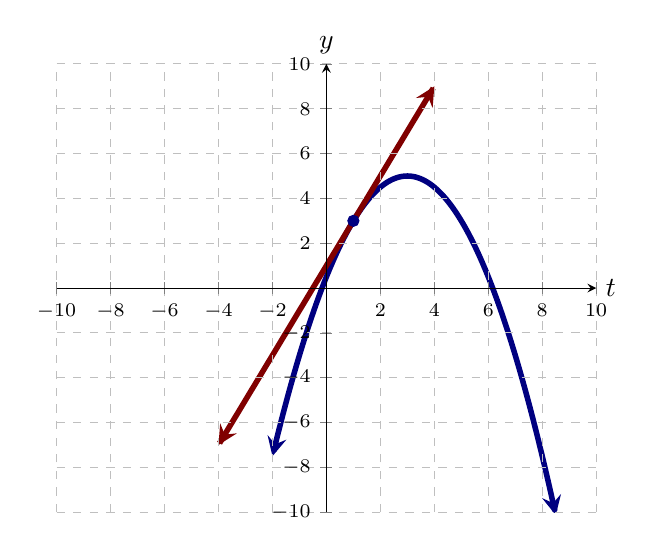
\begin{tikzpicture}
  \begin{axis}[
            domain=-10:10, ymax=10, xmax=10, ymin=-10, xmin=-10,
            axis lines =center, xlabel=$t$, ylabel={$y$}, grid = major, grid style={dashed},
            ytick={-10,-8,-6,-4,-2,2,4,6,8,10},
            xtick={-10,-8,-6,-4,-2,2,4,6,8,10},
            yticklabels={$-10$,$-8$,$-6$,$-4$,$-2$,$2$,$4$,$6$,$8$,$10$}, 
            xticklabels={$-10$,$-8$,$-6$,$-4$,$-2$,$2$,$4$,$6$,$8$,$10$},
            ticklabel style={font=\scriptsize},
            every axis y label/.style={at=(current axis.above origin),anchor=south},
            every axis x label/.style={at=(current axis.right of origin),anchor=west},
            axis on top
          ]
          
          %\addplot [line width=2, penColor2, smooth,samples=100,domain=(-6:2)] {-2*x-3};
          \addplot [line width=2, penColor, smooth,samples=200,domain=(-2:8.5),<->] {-0.5*(x-3)^2 + 5};
          \addplot [line width=2, penColor2, smooth,samples=200,domain=(-4:4),<->] {2*(x-1)+3};

          %\addplot[color=penColor,fill=penColor2,only marks,mark=*] coordinates{(-6,9)};
          %\addplot[color=penColor,fill=penColor2,only marks,mark=*] coordinates{(2,-7)};

          \addplot[color=penColor,fill=penColor,only marks,mark=*] coordinates{(1,3)};
          %\addplot[color=penColor,fill=penColor,only marks,mark=*] coordinates{(-0.162,0)};
          %\addplot[color=penColor,fill=penColor,only marks,mark=*] coordinates{(6.162,0)};



           

  \end{axis}
\end{tikzpicture}
\end{image}










\begin{center}
\textbf{\textcolor{green!50!black}{ooooo-=-=-=-ooOoo-=-=-=-ooooo}} \\

more examples can be found by following this link\\ \link[More Examples of Quadratic Functions]{https://ximera.osu.edu/csccmathematics/precalculus2/precalculus2/quadraticFunctions/examples/exampleList}

\end{center}




\end{document}
